\begin{figure}[htbp!]
    \centering
    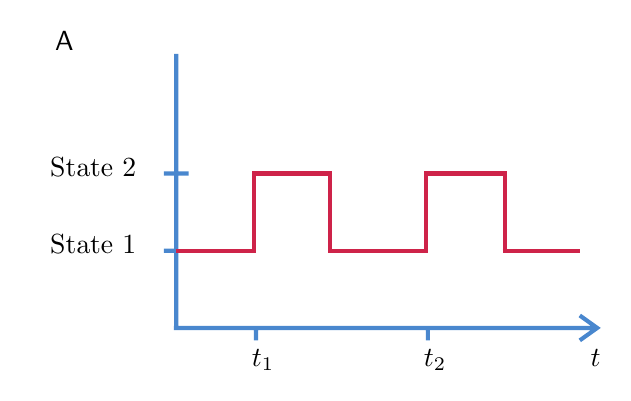
\begin{tikzpicture}[x=0.9pt,y=0.9pt,yscale=-1,xscale=1]
        \path (20,200); %set diagram left start at 0, and has height of 200

        \draw [color={rgb, 255:red, 73; green, 135; blue, 206 }, draw opacity=1 ][line width=1.5][-]
        % axes
        (78.67,210.33) -- (248.67,210.33)
        (79.67,100.33) -- (79.67,210.33)

        % arrow
        (241.67,205.33) -- (248.67,210.33) -- (241.67,215.33)
        %(74.67,105.33) -- (79.67,100.33) -- (84.67,105.33)

        % axis ticks
        (111.67, 210.33) -- (111.67, 215.33)
        (180.67, 210.33) -- (180.67, 215.33)
        (74.67,179.33) -- (79.67,179.33)
        (74.67,148.33) -- (84.67,148.33);
        \draw;

        \draw [color={rgb, 255:red, 206; green, 35; blue, 73 }, draw opacity=1 ][line width=1.5][-]

        (79.67,179.33) -- (111.67,179.33)
        (110.85,179) -- (110.85,147.50)
        (111.67,148.33) -- (140.67,148.33)
        (141.49,147.50) -- (141.49,179)
        (140.67,179.33) -- (180.67,179.33)
        
        (179.85,179) -- (179.85,147.50)
        (180.67,148.33) -- (210.67,148.33)
        (211.49,147.50) -- (211.49,179)
        (210.67,179.33) -- (241.67,179.33);
        \draw;

        \draw [-] (30,90) node [anchor=north west][inner sep=0.75pt] [align=left] {\textsf{A}};
        \draw [-] (28,172) node [anchor=north west][inner sep=0.75pt] [align=left] {State 1};
        \draw [-] (28,141) node [anchor=north west][inner sep=0.75pt] [align=left] {State 2};
        \draw [-] (109,218) node [anchor=north west][inner sep=0.75pt] [align=left] {$t_1$};
        \draw [-] (178,218) node [anchor=north west][inner sep=0.75pt] [align=left] {$t_2$};
        \draw [-] (245,218) node [anchor=north west][inner sep=0.75pt] [align=left] {$t$};

    \end{tikzpicture}
    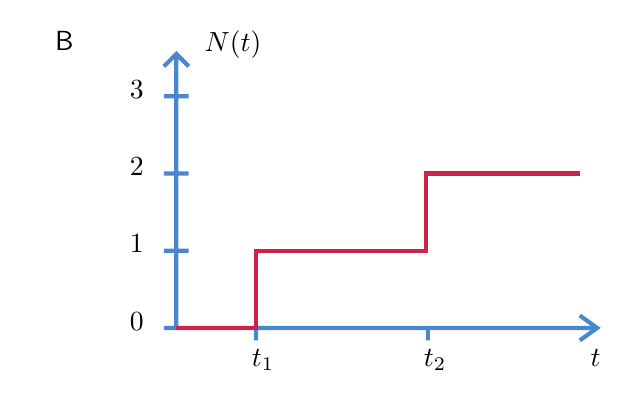
\begin{tikzpicture}[x=0.9pt,y=0.9pt,yscale=-1,xscale=1]
        \path (20,200); %set diagram left start at 0, and has height of 200

        \draw [color={rgb, 255:red, 73; green, 135; blue, 206 }, draw opacity=1 ][line width=1.5][-]
        % axes
        (78.67,210.33) -- (248.67,210.33)
        (79.67,100.33) -- (79.67,210.33)

        % arrow
        (241.67,205.33) -- (248.67,210.33) -- (241.67,215.33)
        (74.67,105.33) -- (79.67,100.33) -- (84.67,105.33)

        % axis ticks
        (111.67, 210.33) -- (111.67, 215.33)
        (180.67, 210.33) -- (180.67, 215.33)

        (74.67,210.33) -- (79.67,210.33)
        (74.67,179.33) -- (84.67,179.33)
        (74.67,148.33) -- (84.67,148.33)
        (74.67,117.33) -- (84.67,117.33);
        \draw;

        \draw [color={rgb, 255:red, 206; green, 35; blue, 73 }, draw opacity=1 ][line width=1.5][-]

        (79.67,210.33) -- (111.67,210.33)
        (111.67,211.15) -- (111.67,178.50)
        (111.67,179.33) -- (180.67,179.33)
        
        (179.85,179) -- (179.85,147.5)
        (180.67,148.33) -- (241.67,148.33);
        \draw;

        \draw [-] (30,90) node [anchor=north west][inner sep=0.75pt] [align=left] {\textsf{B}};
        \draw [-] (60,203) node [anchor=north west][inner sep=0.75pt] [align=left] {0};
        \draw [-] (60,172) node [anchor=north west][inner sep=0.75pt] [align=left] {1};
        \draw [-] (60,141) node [anchor=north west][inner sep=0.75pt] [align=left] {2};
        \draw [-] (60,110) node [anchor=north west][inner sep=0.75pt] [align=left] {3};
        \draw [-] (109,218) node [anchor=north west][inner sep=0.75pt] [align=left] {$t_1$};
        \draw [-] (178,218) node [anchor=north west][inner sep=0.75pt] [align=left] {$t_2$};
        \draw [-] (90,90) node [anchor=north west][inner sep=0.75pt] [align=left] {$N(t)$};
        \draw [-] (245,218) node [anchor=north west][inner sep=0.75pt] [align=left] {$t$};

    \end{tikzpicture}
    \caption[Example of transitions in a multi-state process and the corresponding counting process]{Example of transitions between two states in a multi-state process (panel A), and the corresponding counting process for the State 1 $\rightarrow$ State 2 transition (panel B).}\label{fig:counting-process}
\end{figure}